\section{Unsaturated consolidation}

\subsection{Theory}

\subsubsection{Fluid mass balance}

The general fluid mass balance equation for unsaturated flow in a deformable porous medium is
%
\begin{eqnarray}
n S^l \dot\rho^l
+
n \rho^l \dot S^l
+
n S^l \rho^l \v^{ls}
+
S^l \rho^l \nabla\cdot\v^s
+
S^l \rho^l \frac{1-n}{\rho^s} \dot\rho^s
=
\nonumber \\
Q_\rho^l + S^l \frac{\rho^l}{\rho^s} Q_\rho^s
\label{eqn:uc1}
\end{eqnarray}
%
Hereby, the basic assumption of Richards type models is that the gaseous phase is immobile, i.e. $\v^g=0$.
Assuming grain incompressibility for isothermal conditions (i.e. $\dot\rho^s=0$) and no solid sources (e.g. resulting from chemical reactions) as well as
applying the constitutive equations for fluid compressibility, capillary pressure, and Darcy flux,
we obtain the following Richards equation for an unsaturated deformable porous medium.
%
\begin{eqnarray}
n S^l \rho_0^l \beta_p \dot p^l
-
n \rho^l \frac{dS^l}{d p_c} \dot p^l
-
\nabla
\left(
\dfrac{\RelKa^l\per}{\mu^l}(\nabla p^l - \dens\grv)
\right)
+
S^l \rho^l \nabla\cdot \dot\u^s
=
Q_\rho^l
\label{eqn:uc2}
\end{eqnarray}
%
Rearrangement with respect to the primary variables $p^l, \u^s$ yields
%
\begin{eqnarray}
\left(
-
n \rho^l \frac{dS^l}{d p_c}
+
n S^l \rho_0^l \beta_p
\right)
\dot p^l
-
\nabla
\left(
\dfrac{\RelKa^l\per}{\mu^l} \nabla p^l
\right)
+
S^l \rho^l \nabla\cdot \dot\u^s
=
\nonumber\\
Q_\rho^l
+
\nabla
\left(
\dfrac{\RelKa^l\per}{\mu^l}\dens\grv
\right)
\label{eqn:uc2}
\end{eqnarray}
%

A constitutive equation, the water content function obtained by experiments, characterizes the relationship between $p^l$ and $\sat^l$ and therefore the derivative $dS^l/dp_c$.

\subsubsection{Momentum balance}

The deformation process is described by the momentum balance equation for the unsaturated porous medium in terms of stresses.

\begin{eqnarray}
\nabla\cdot
(\s - \alpha_b S^l p^l \bf I) + \rho\g = 0
\label{eqn:mb_us}
\end{eqnarray}

All symbols are denoted in chapter \ref{sec:symbols}.
%

\subsubsection{Numerical scheme}

The standard Galerkin finite element approach is applied for the numerical solution of the PDEs (\ref{eqn:uc2}) and (\ref{eqn:mb_us}) resulting into the following system of algebraic equations.

\begin{eqnarray}
\underbrace{
\left[
\begin{array}{ll}
\mathbf{C}_{pp} & \mathbf{C}_{pu}
\\
\mathbf{C}_{up} & \mathbf{C}_{uu}
\end{array}
\right]
}_{\mathbf C}
%
\frac{d}{dt}
\underbrace{
\left\{
\begin{array}{l}
\hat\PressureVec^l
\\
\hat\Disp^s
\end{array}
\right\}
}_{\mathbf x}
%
+
%
\underbrace{
\left[
\begin{array}{ll}
\mathbf{K}_{pp} & \mathbf{K}_{pu}
\\
\mathbf{K}_{up} & \mathbf{K}_{uu}
\end{array}
\right]
}_{\mathbf K}
%
\left\{
\begin{array}{l}
\hat\PressureVec^l
\\
\hat\Disp^s
\end{array}
\right\}
%
=
\underbrace{
\left\{
\begin{array}{l}
\mathbf{r}_p
\\
\mathbf{r}_u
\end{array}
\right\}
}_{\mathbf{r}}
\nonumber
\\
\end{eqnarray}

where $\C_{up}, \C_{uu}, \K_{pu}$ are zero.

\begin{eqnarray}
\left[
\begin{array}{cc}
\mathbf{C}_{pp} & \mathbf{C}_{pu}
\\
\mathbf{0} & \mathbf{0}
\end{array}
\right]
%
\frac{d}{dt}
\left\{
\begin{array}{l}
\hat\PressureVec^l
\\
\hat\Disp^s
\end{array}
\right\}
%
+
%
\left[
\begin{array}{ll}
\mathbf{K}_{pp} & \mathbf{0}
\\
\mathbf{K}_{up} & \mathbf{K}_{uu}
\end{array}
\right]
%
\left\{
\begin{array}{l}
\hat\PressureVec^l
\\
\hat\Disp^s
\end{array}
\right\}
%
=
\left\{
\begin{array}{l}
\mathbf{r}_p
\\
\mathbf{r}_u
\end{array}
\right\}
\nonumber
\\
\end{eqnarray}

%------------------
Time discretization with explicit finite differences yields

\begin{eqnarray}
\left(
\frac{1}{\Delta t} \C_{pp} + \theta \K_{pp}
\right)
\hat{\p}^l_{n+1}
+
\frac{1}{\Delta t} \C_{pu}
\hat\u^s_{n+1}
\nonumber\\
=
\left(
\frac{1}{\Delta t} \C_{pp} + (1-\theta) \K_{pp}
\right)
\hat\p^l_{n}
+
\frac{1}{\Delta t} \C_{pu}
\hat\u^s_{n}
+
\r_p
\end{eqnarray}

%------------------

\begin{eqnarray}
\theta \K_{up}
\hat\p^l_{n+1}
+
\theta \K_{uu}
\hat\u^s_{n+1}
\nonumber\\
=
(1-\theta) \K_{up}
\hat\p^l_{n+1}
+
(1-\theta) \K_{pp}
\hat\u^s_{n+1}
+
\r_u
\end{eqnarray}

%------------------

with following finite element matrices

\begin{eqnarray}
%---
\C^e_{pp}
&=&
\int_{\Domain^e}
\SFVPressure^T
\left[
- n \rho^l \frac{dS^l}{dp_c}
+
n S^l \rho_0^l \beta_p
%\UnitOperator^T\GradOperator
\right]
\SFVPressure
\,
d\Domain^e
\nonumber
\\
%---
\K^e_{pp}
&=&
\int_{\Domain^e}
\nabla\SFVPressure^T
\left[
- \dfrac{\RelKa^l\per}{\mu^l}
\right]
\nabla\SFVPressure
\,
d\Domain^e
\nonumber
\\
%---
\C^e_{pu}
&=&
\int_{\Domain^e}
\SFVPressure^T
\left[
S^l \rho^l
\right]
\nabla\TFVDisp
\,
d\Domain^e
%\nonumber
\\
%---
\r^e_{p}
&=&
\int_{\Domain^e}
\left[
Q^l_\rho
\right]
\SFVPressure
\,
d\Domain^e
+
\int_{\Domain^e}
\SFVPressure^T
\left[
\dfrac{\RelKa^l\per}{\mu^l} \rho^l \g
\right]
\nabla\SFVPressure
\,
d\Domain^e
\nonumber
\end{eqnarray}

%------------------

\begin{eqnarray}
%---
\K^e_{up}
&=&
\int_{\Domain^e}
\B^T
\left[
\alpha_b S^l
\right]
\m\SFVPressure
\,
d\Domain^e
\nonumber
\\
%---
\K^e_{uu}
&=&
\int_{\Domain^e}
\B^T
\left[
\mathbb C
\right]
\B
\,
d\Domain^e
\nonumber
\\
%---
\r^e_{u}
&=&
\int_{\Domain^e}
\TFVDisp
\left[
\rho\g
\right]
\,
d\Domain^e
\end{eqnarray}

where m is a mapping vector as
\[\m = [1\, 1\, 1\, 0]^T\] 
for plane strain problems and
\[\m = [1\, 1\, 1\, 0\, 0\, 0]^T\] for 3D problems
%%%%%%%%%%%%%%%%%%%%%%%%%%%%%%%%%%%%%%%%%%%%%%%%%%%%%%%%%%%%%%%%%%%%%%%%%%


\subsection{Liakopoulos Experiment}
\label{sec:Liakopoulos} \index{example - Liakopoulos}

\subsubsection*{Problem definition}
The first example
is a drainage test
based on an experiment by Liakopoulos (1965).
Desaturation takes place due to gravitational effects.
This example was studied previously by several authors,
e.g.
Liakopoulos (1965),
Narasimhan \& Witherspoon (1978),
Zienkiewicz et al. (1990),
Schrefler \& Zhan (1993).
Therefore, this example is well suited as benchmark,
moreover, because of the lack of any analytical solutions
for this type of coupled, non-linear problems.
In this test example,
multiphase flow in a deforming porous medium is studied.
At first we employ the Richards approximation,
i.e. air remains at atmospheric pressure.

The physical experiment of Liakopoulos was conducted in a column
packed with so-called Del Monte sand. Moisture content and tension
at several points along the column were measured with tensiometers
(Fig. \ref{fig:liakop1}, Fig. \ref{fig:liakop2}).

% *** EPS-Grafik ***
\begin{figure}[htb!]
\begin{center}
\footnotesize
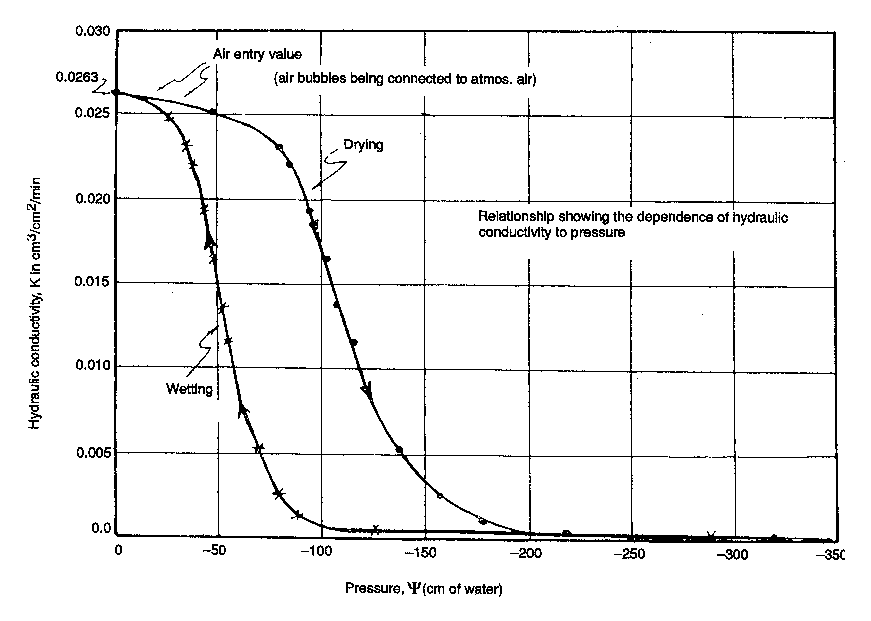
\includegraphics[width=0.6\columnwidth]{HM/HM_unsat/liakop1.eps}  % Filename.eps
\caption{Hydraulic conductivity vs pressure,
with $K = k\Density\Gravity/\Viscosity$ and $\Psi = \Pressure/\Density\Gravity$
(Liakopoulos 1965)
}
\label{fig:liakop1}
\end{center}
\end{figure}
%

% *** EPS-Grafik ***
\begin{figure}[htb!]
\begin{center}
\footnotesize
\includegraphics[width=0.5\columnwidth]{HM/HM_unsat/liakop2.eps}  % Filename.eps
\caption{Hydraulic head vs water content,
with
$\Psi = \Pressure/\Density\Gravity$
and
$\MoistureContent = \Porosity\Saturation$
(Liakopoulos 1965)
}
\label{fig:liakop2}
\end{center}
\end{figure}
%

In the simulation, the column is assumed has size of $0.1m\times1m$ and discretized into 20 quadrilateral elements (Fig. \ref{fig:modelia}).

\subsubsection*{Initial and boundary conditions}
Based on the experiment, we assume that the initial pressure is zero everywhere in the domain.
Boundary conditions for both fluid and displacement fields is depicted in Fig. \ref{fig:modelia}.
\begin{figure}[!htb]
\begin{center}
\footnotesize
\input{HM/HM_unsat/liako.eepic}
\caption{Boundary conditions}
\label{fig:modelia}
\end{center}
\end{figure}
%
Such initial boundary conditions imply that the sample in fully saturated at the beginning, the water is allowed to
flow out from the bottom boundary.

\subsubsection*{Material properties}
The capillary pressure $\CapillaryPressure(\Saturation)$
\begin{eqnarray}
\CapillaryPressure
=
\left(
\frac{1-\Saturation}{1.9722}
\times 10^{11}
\right)^{\frac{1}{2.4279}}
\label{eq:hm_sat_p_s}
\end{eqnarray}
as well as the relative permeability relationships
$\PermRelP(\Saturation)$
\begin{eqnarray}
\PermRelP
=
1 - 2.207
(1-\Saturation)^{1.0121}
\label{eq:hm_sat_rs}
\end{eqnarray}
fit the measured data for saturations larger than 0.84. The physical parameter are given in the table below.
%

 \begin{table}[!htb]
\centering
\begin{tabular}{lll}
\hline\hline\noalign{\smallskip}
Property & Value & Unit \\
\noalign{\smallskip}\hline\noalign{\smallskip}
Young's modulus, $E$  &  $MPa$   &  1.3   \\
Poisson's ratio,  $\nu$  & -- &  0.4 \\
Solid grain density, $\Density^s$  &$kg m^{-3}$ & $2000$ \\
Liquid density, $\Density^l$       &$kg m^{-3}$ & $kg m^{-3}$ \\
Porosity, $\Porosity$            & --  & $0.2975$ \\
Permeability, $\Perm$         & $ m^2$     & $4.5\times 10^{-13}$ \\
Water viscosity,  $\mu$      & $Pa s$     & $10^{-3} $ \\
Gravity,   $\Gravity$    &  $m s^{-2}$ & $9.806 $ \\
capillary pressure $\CapillaryPressure(\Saturation)$   &  $Pa$ & eqn. (\ref{eq:hm_sat_p_s}) \\
Relative permeability, $\PermRelP(\Saturation)$   &  -- & eqn. (\ref{eq:hm_sat_rs})\\
\noalign{\smallskip}\hline\hline
\end{tabular}
\caption{Material parameters}
\label{tab:hm_sat}
\end{table}




%The boundary conditions are illustrated in the below figure.

\subsubsection*{Results}

We conduct two kinds of simulation such as:
 one is taking account of the gravity force as a load for displacement field, while the other ignore the the gravity force.

For the case of non-gravity force, Fig. \ref{fig_HM_sat_nog} shows history profile of water pressure
$\Pressure$, water saturation $\Saturation$, vertical solid
displacement $u_y$ and vertical stress $\stress_{yy}$.
\begin{figure}[!htb]
  \begin{center}
  \epsfig{figure=HM/HM_unsat/pre_nog.eps,height=0.49\textwidth, width=0.49\textwidth}
  \epsfig{figure=HM/HM_unsat/sat_nog.eps,height=0.49\textwidth, width=0.49\textwidth}
  \epsfig{figure=HM/HM_unsat/uy_nog.eps,height=0.49\textwidth, width=0.49\textwidth}
  \epsfig{figure=HM/HM_unsat/syy_nog.eps,height=0.49\textwidth, width=0.49\textwidth}
  \end{center}
\caption{Simulated results (without gravity force), $\Pressure$, $\Saturation$,
 $u_y$, $\stress_{yy}$ }
  \label{fig_HM_sat_nog}
\end{figure}
Results of $\Pressure$, water saturation $\Saturation$, vertical solid
displacement $u_y$ agree with what given in \cite{LewSch:98} (see pages 167-172).


The vertical profile of results obtained by taking account of the gravity force are shown in Fig. \ref{fig_HM_sat_g}.
If compare the saturation result with that obtained by ignoring the gravity fore, one can easily find the
 desaturated procedure is enhanced apparently. This highlights the impact of displacement to water pressure and
  the coupling effects.
\begin{figure}[!htb]
  \begin{center}
  \epsfig{figure=HM/HM_unsat/pre_g.eps,height=0.49\textwidth, width=0.49\textwidth}
  \epsfig{figure=HM/HM_unsat/sat_g.eps,height=0.49\textwidth, width=0.49\textwidth}
  \epsfig{figure=HM/HM_unsat/uy_g.eps,height=0.49\textwidth, width=0.49\textwidth}
  \epsfig{figure=HM/HM_unsat/syy_g.eps,height=0.49\textwidth, width=0.49\textwidth}
  \end{center}
\caption{Simulated results (with gravity force), $\Pressure$, $\Saturation$,
 $u_y$, $\stress_{yy}$}
  \label{fig_HM_sat_g}
\end{figure}

Benchmark deposit

\begin{tabular}{|l|l|l|}
  \hline
  Benchmark & Problem type & Path in benchmark deposit \\
  \hline
 \emph{hm\_unsat}& HM & benchmarks\verb\HM\ \\
  \hline
\end{tabular}
%%%%%%%%%%%%%%%%%

